\documentclass{beamer}
\usepackage[T1]{fontenc}
\usepackage{listings}

\graphicspath{{../figures/}}

%\title{PowerEnJoy}
%\subtitle{Design Document}
%\author{Patrizia Porati \\ Tommaso Sardelli}
%\date{\today}
%\usetheme{CambridgeUS}

\usetheme[pageofpages=of,% String used between the current page and the total page count.
          titleline=true,% Show a line below the frame title.
          alternativetitlepage=true,% Use the fancy title page.
         ]{Torino}

%\author{\texorpdfstring{Tommaso Sardelli\newline\tiny\url{tommaso.sardelli[at]mail.polimi.it}}{Author}}
\author{Patrizia Porati \newline Tommaso Sardelli}
\title{PowerEnJoy}
\subtitle{Design Document}
\institute{Politecnico di Milano}
\date{\today}

\begin{document}
	
\begin{frame}[t,plain]
    \titlepage
\end{frame}

%--------------
% SCOPE 
%--------------
\begin{frame}
    \frametitle{Scope}
    \begin{itemize}
        \item \textbf{Intended audience:} project managers and software developers 
            \pause
        \item Architectural choices and paradigms
            \pause
        \item \textbf{Assumption:} the system will not be implemented by our team
            \pause
        \item No fixed constraints for future implementers
    \end{itemize}
\end{frame}

%-------------
% MAIN PRINCIPLES
%-------------
\begin{frame} {Main Principles}
    \begin{itemize}
        \item \textbf{Client-Server} model.
        \item \textbf{RESTful} API.
        \item \textbf{Microservices} approach.
    \end{itemize}
\end{frame}

%--------------
% CLIENT-SERVER
%--------------
\begin{frame}{Client-Server}
    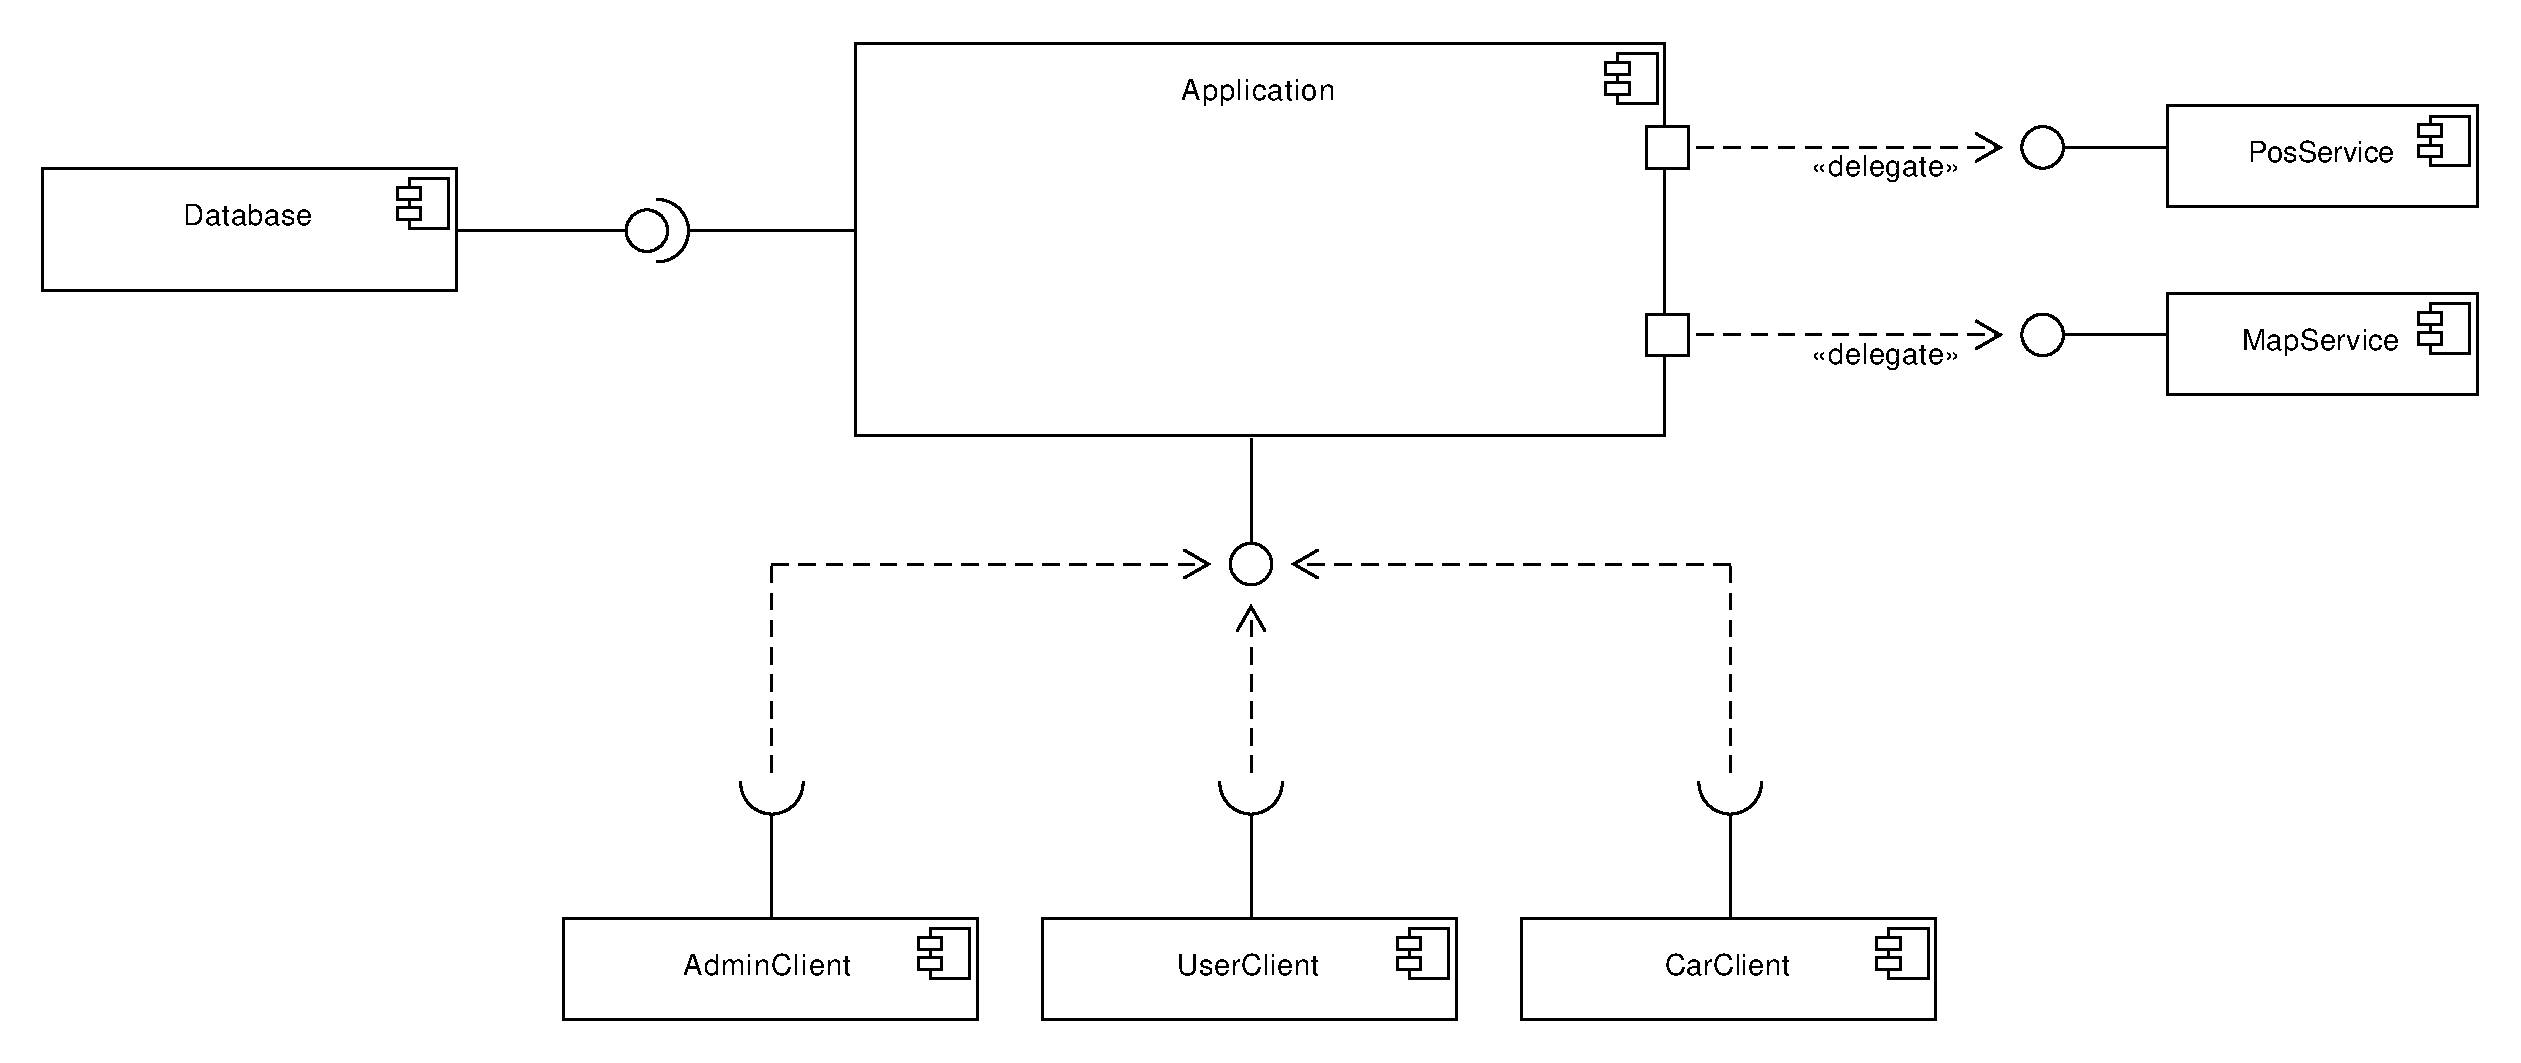
\includegraphics[width=0.9\textwidth]{high_level_components}
\end{frame}

%--------------
% RESTful
%--------------
\begin{frame}{RESTful API}
    \begin{itemize}
        \item Intuitiveness
        \item Simplicity
        \item Modifiability
        \item Scalability
        \item Performance
    \end{itemize}
\end{frame}

\begin{frame}[fragile]
    \frametitle{REST Simplicity}
    \textbf{Syntax:} /resource/identifier/resource

    \begin{lstlisting}

        GET /users/5678/rides 
        GET /cars/1234/reservations 

        POST /users/5678/reservations?car=1234 
    \end{lstlisting}
\end{frame}

%--------------
% Microservices
%--------------
\begin{frame}{Microservices}
    \textbf{PROS:}
    \begin{itemize}
        \item Decoupled
        \item Single Responsibility
        \item Composable
    \end{itemize}
    \vspace{\baselineskip}
    \textbf{CONS:}
    \begin{itemize}
        \item Harder to implement
        \item Side effects (latency, inconsistency)
    \end{itemize}
    \vfill
    Lots of pre-made solutions for different languages
\end{frame}
\begin{frame}{Microservices}
    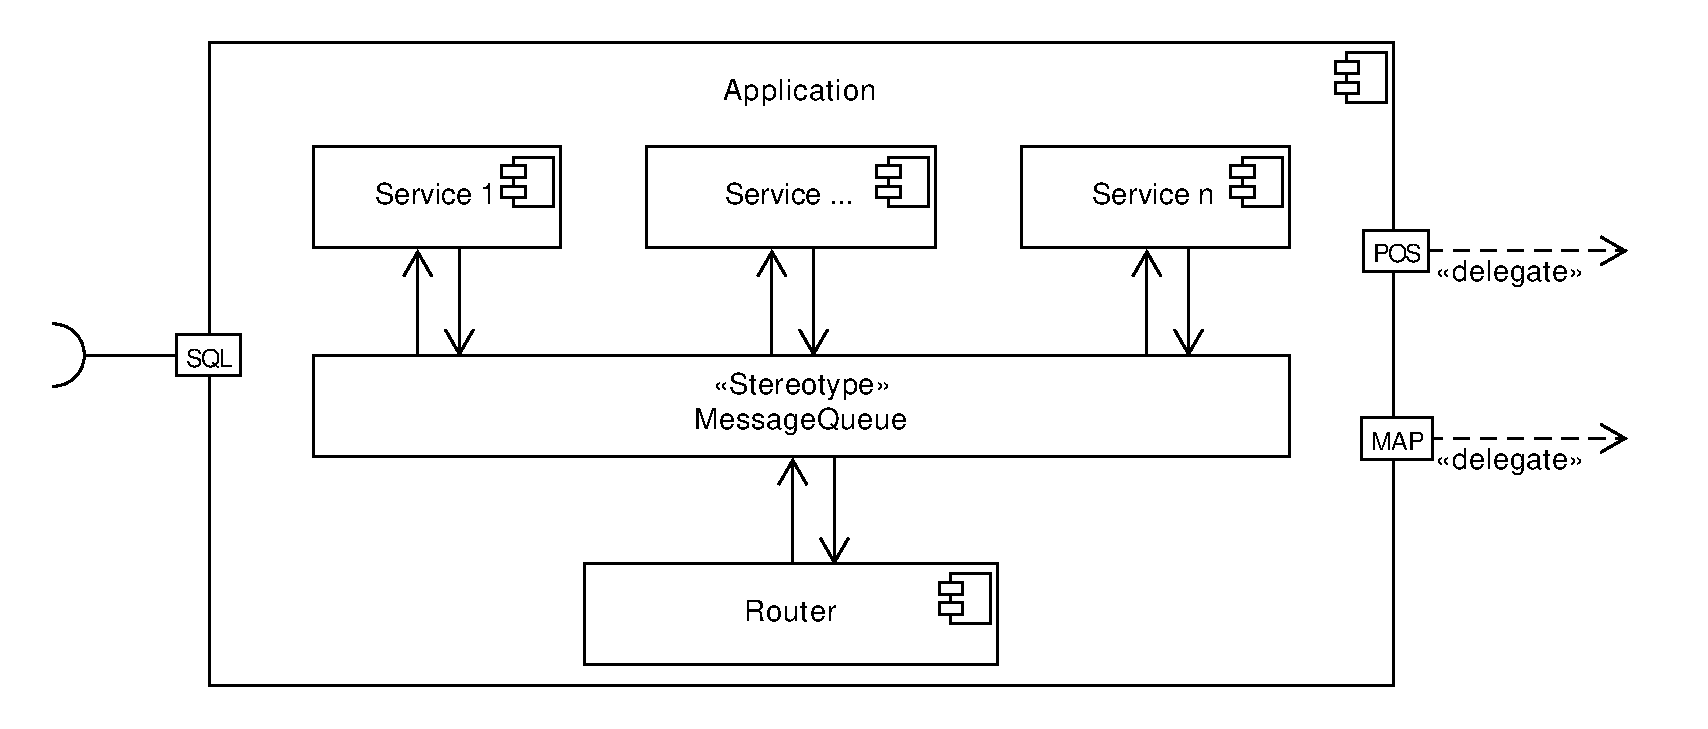
\includegraphics[width=0.9\textwidth]{internal_high_level_components}
\end{frame}

\begin{frame}{Microservices}
    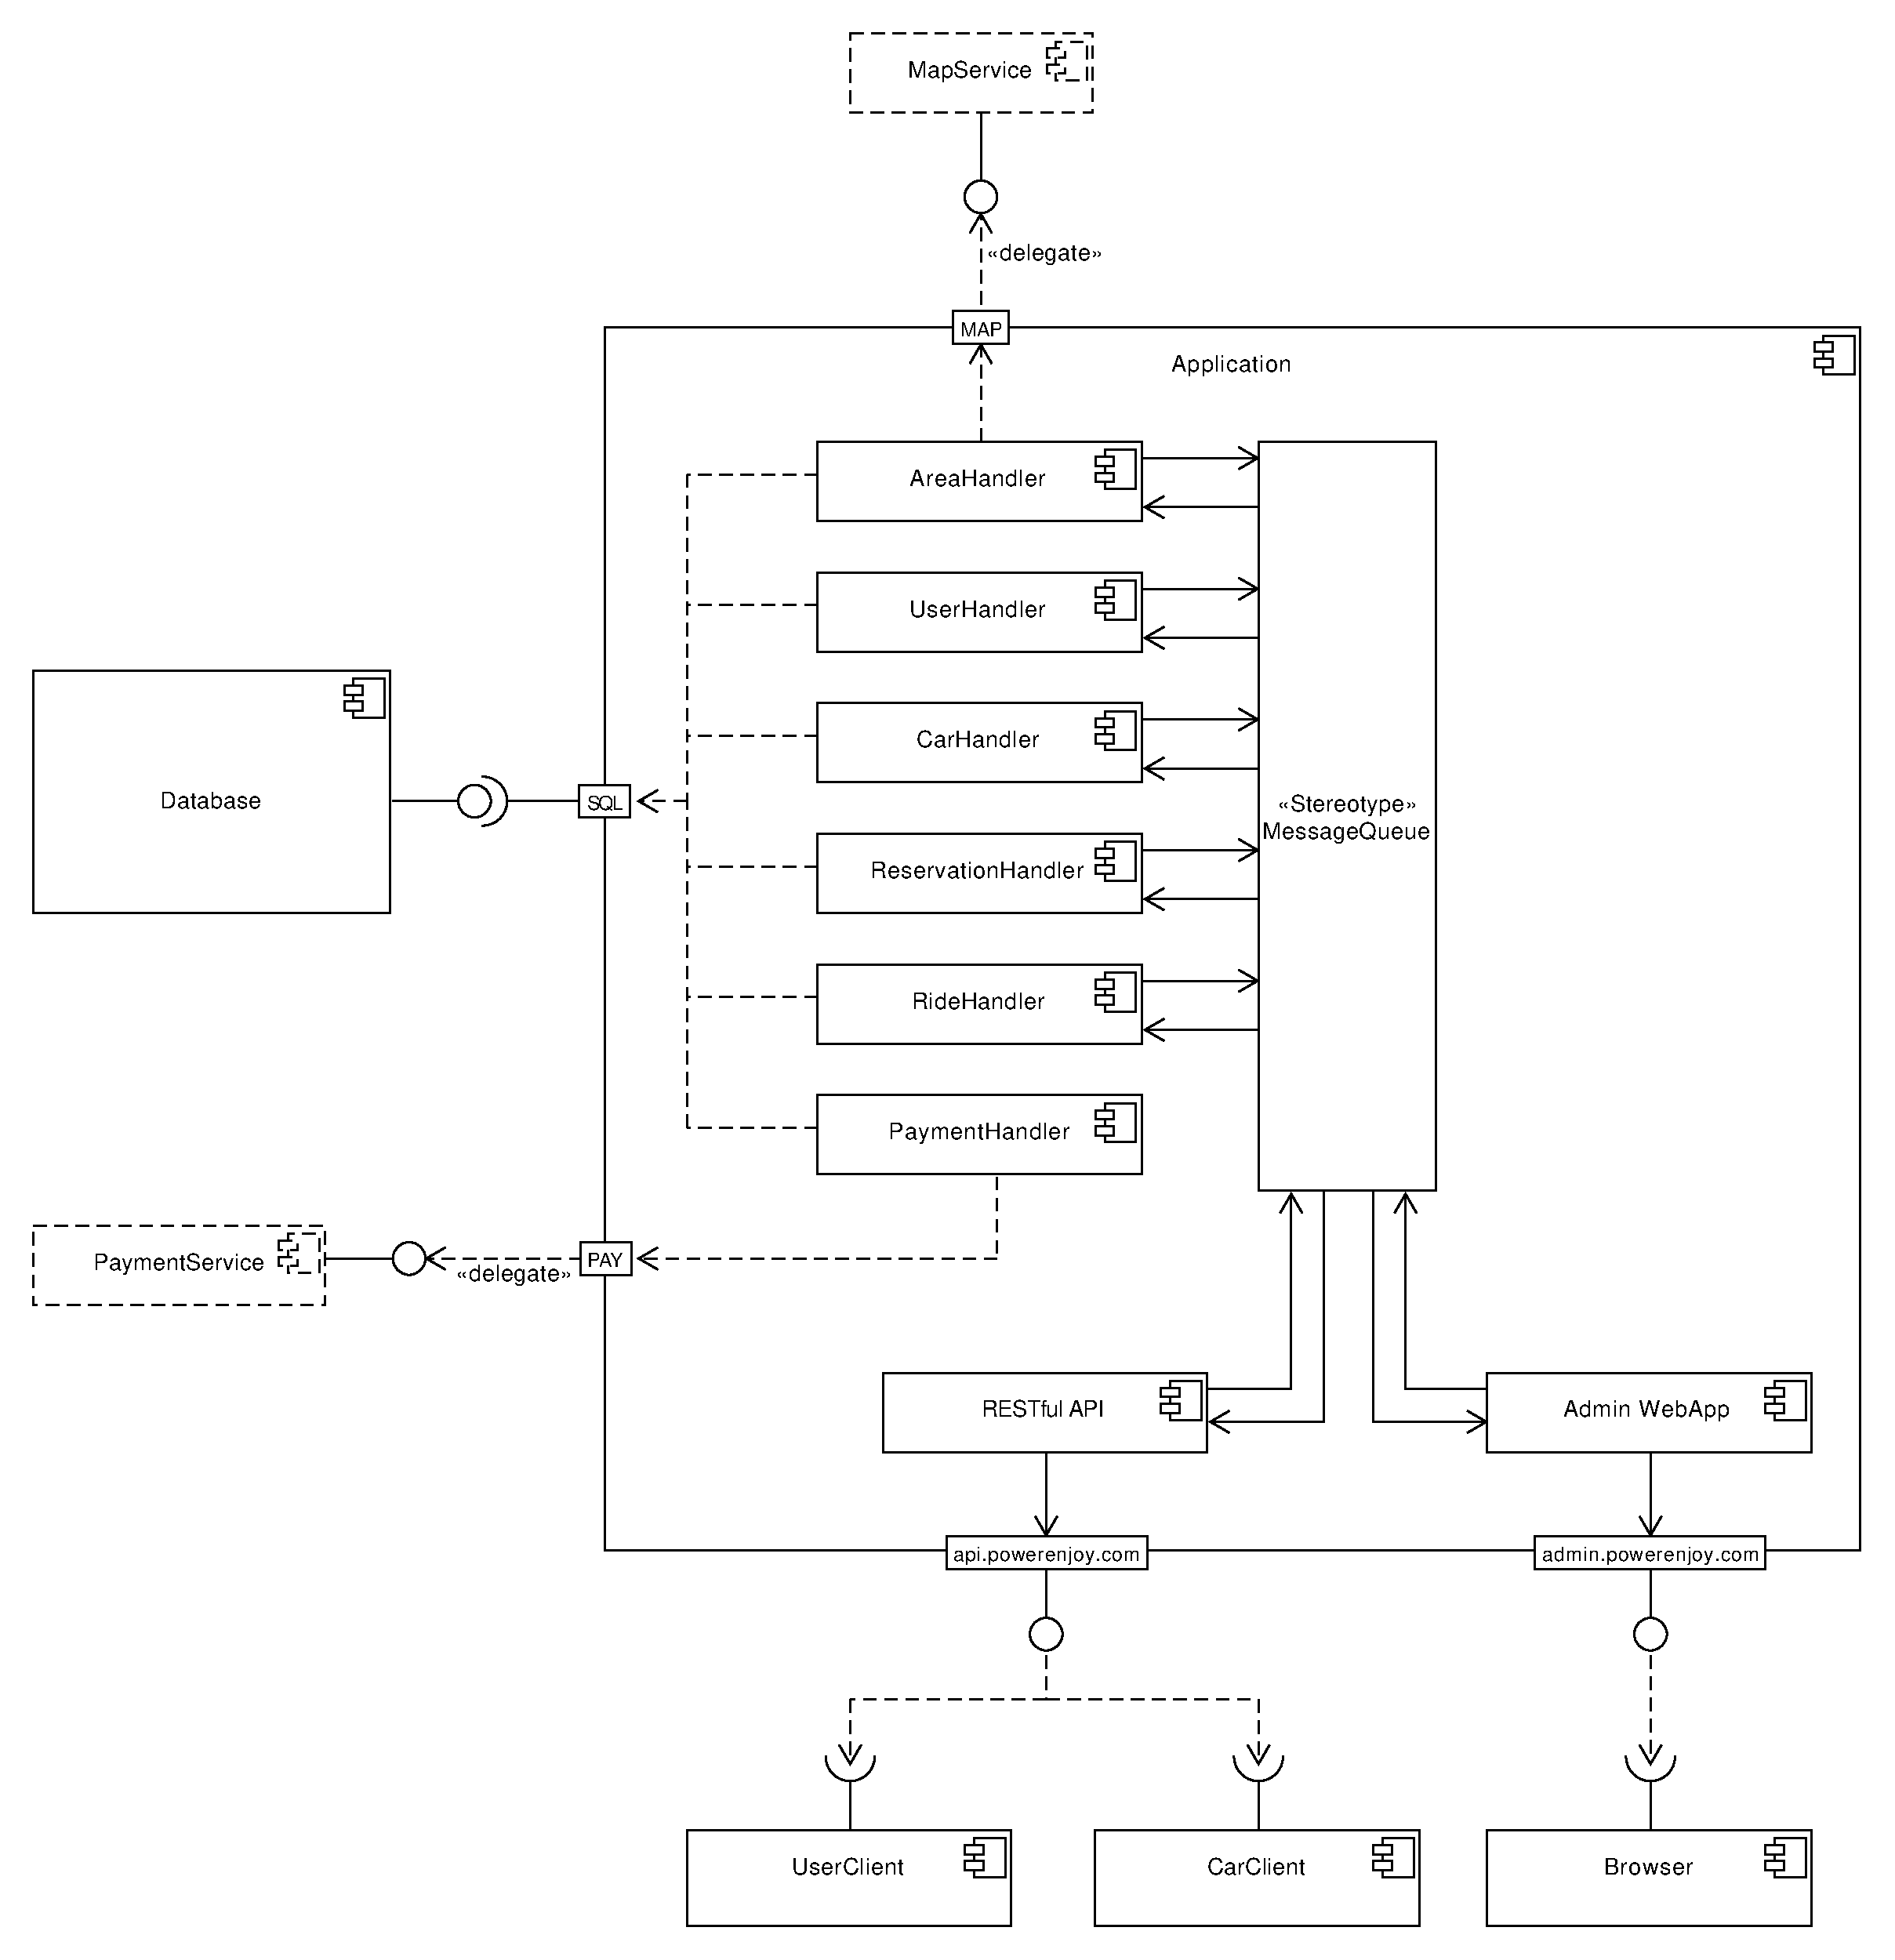
\includegraphics[width=\textwidth]{low_level_components}
\end{frame}

%--------------
% Deployment
%--------------
\begin{frame}{Deployment}
    \begin{itemize}
        \item IaaS
        \item Three-Tier
        \item Single entry point
        \item Start small and grow with requests
    \end{itemize}
\end{frame}

\begin{frame}{Deployment}
    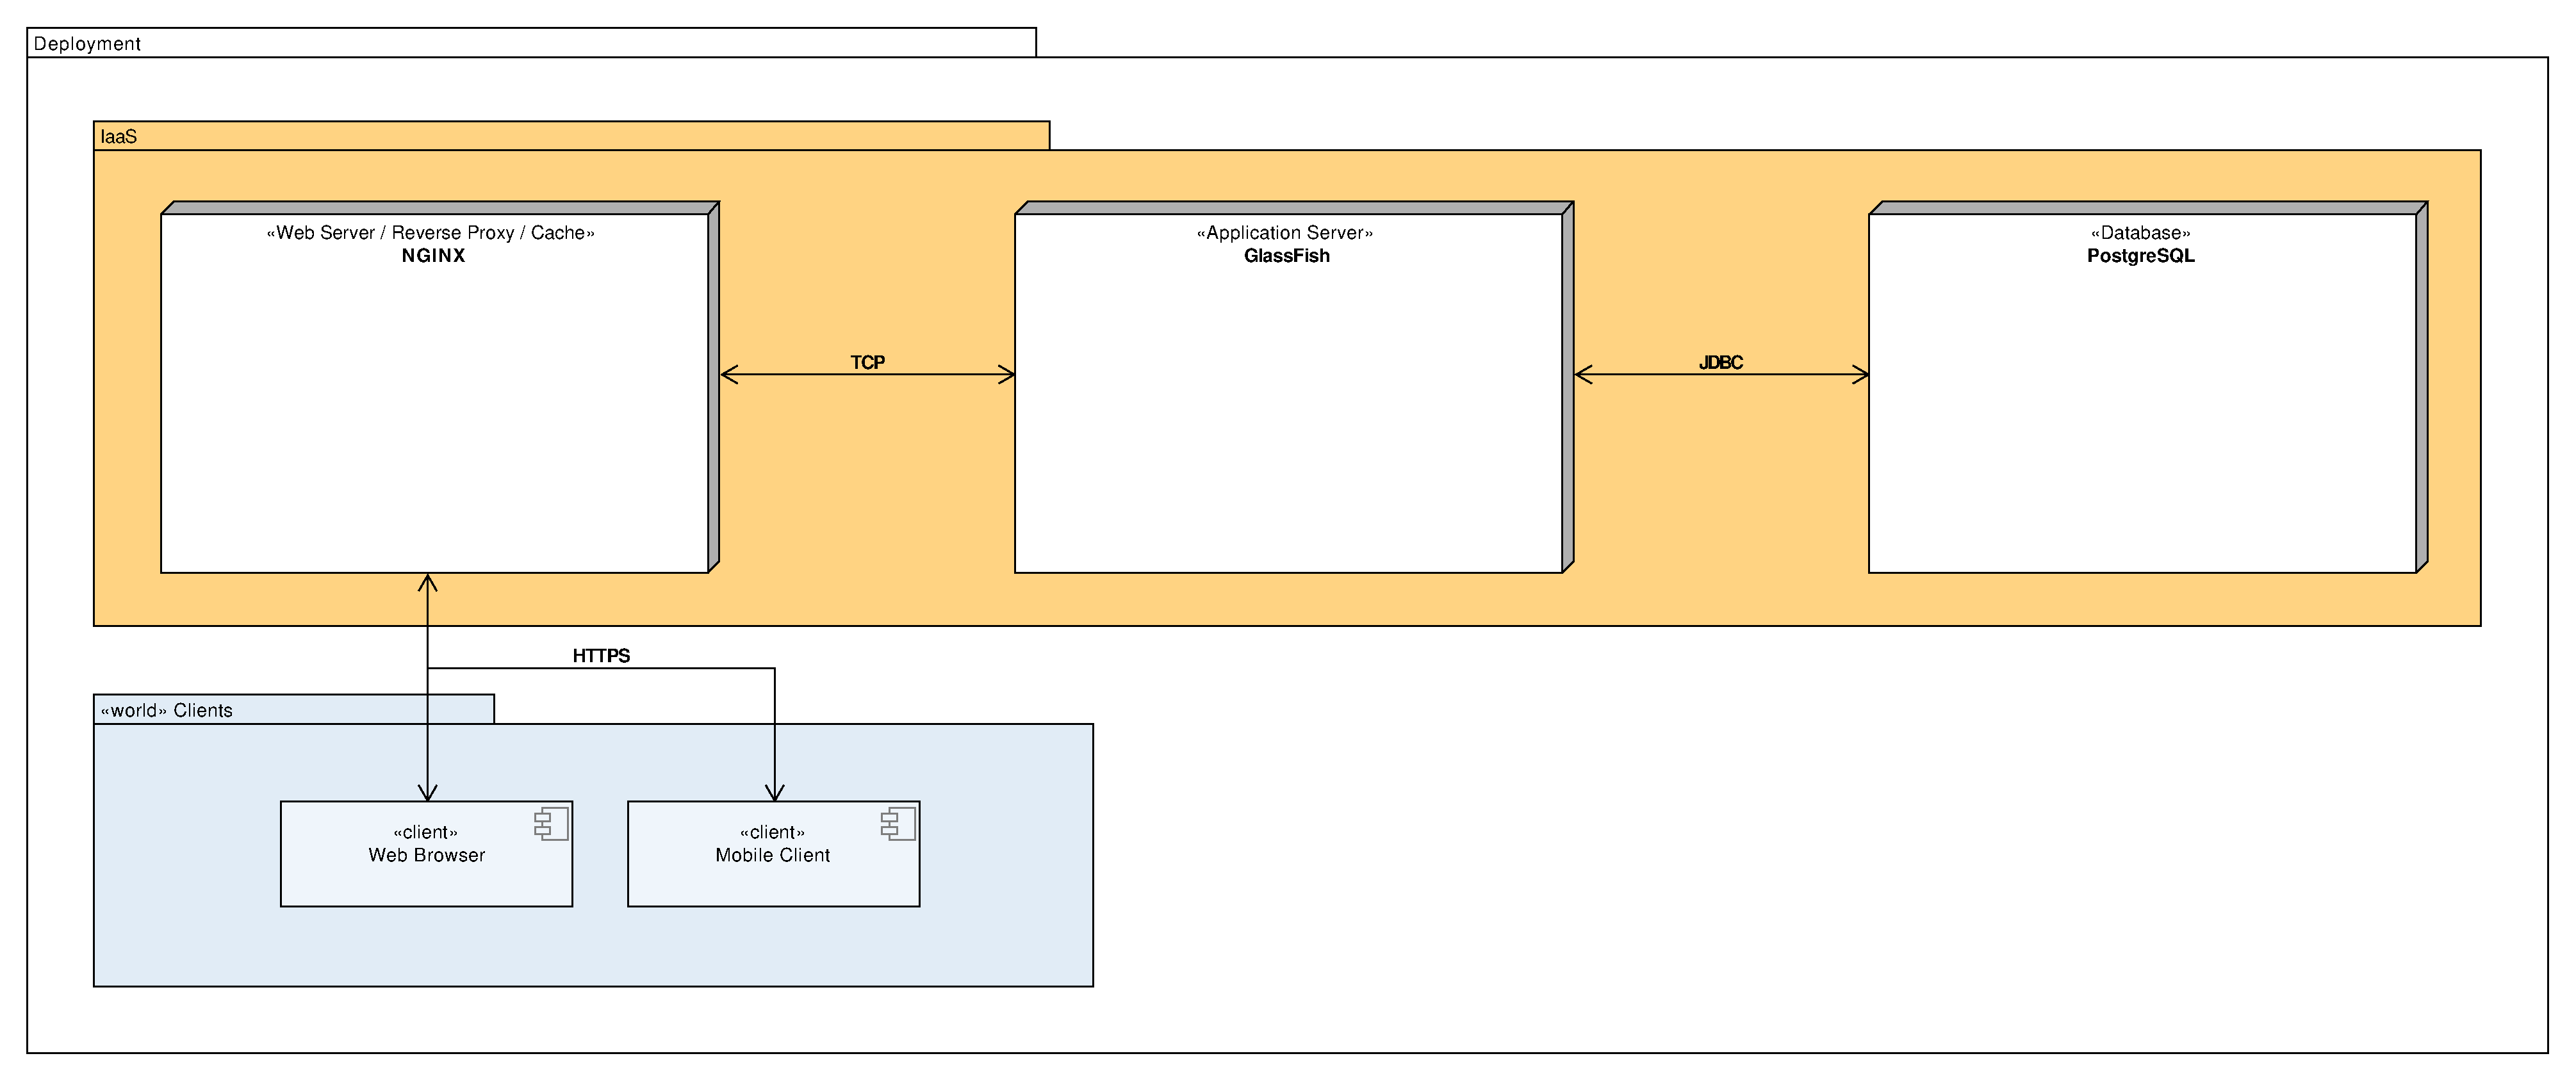
\includegraphics[width=\textwidth]{deployment}
\end{frame}

\end{document}
